\section{Pendahuluan}
\subsection{Latar Belakang}
Mikrokontroler merupakan salah satu komponen penting dalam sistem tertanam (embedded system) yang digunakan untuk mengendalikan perangkat elektronik melalui pemrosesan instruksi program dan interaksi dengan perangkat keras. Mikrokontroler memungkinkan suatu sistem menerima masukan dari sensor atau perangkat input, memproses informasi, serta menghasilkan keluaran untuk mengendalikan perangkat seperti LED dan aktuator.

Dalam pengembangan sistem berbasis mikrokontroler, diperlukan pemahaman mengenai karakteristik perangkat keras, lingkungan pengembangan perangkat lunak, serta cara berkomunikasi dengan perangkat input dan output. Salah satu antarmuka yang umum digunakan adalah General Purpose Input/Output (GPIO), yang memungkinkan mikrokontroler berinteraksi dengan komponen eksternal melalui sinyal digital maupun analog.

Pada praktikum ini digunakan dua jenis development board, yaitu STM32 Blackpill dan ESP32 DevKit. Kedua board tersebut memiliki karakteristik dan lingkungan pemrograman yang berbeda. STM32 Blackpill diprogram menggunakan framework Arduino dengan bantuan ST-Link sebagai perangkat untuk melakukan proses pemrograman, sedangkan ESP32 diperkenalkan menggunakan framework ESP-IDF dan Arduino. Pengembangan program dilakukan melalui Visual Studio Code dengan ekstensi PlatformIO sebagai lingkungan pengembangan terintegrasi.

Selain pengenalan mikrokontroler dan lingkungan pengembangannya, praktikum ini juga membahas konfigurasi GPIO untuk membaca masukan dari pushbutton menggunakan resistor pull-up dan pull-down. Permasalahan floating dan bouncing pada tombol mekanik turut dipelajari karena dapat menyebabkan pembacaan input yang tidak stabil. Selanjutnya, penggunaan GPIO sebagai masukan analog diperkenalkan melalui ADC (Analog-to-Digital Converter) untuk membaca perubahan tegangan dari sensor cahaya LDR (Light Dependent Resistor).

Melalui praktikum ini, diharapkan praktikan dapat memahami dasar pengoperasian mikrokontroler, konfigurasi GPIO, serta pengolahan masukan digital dan analog sebagai dasar dalam pengembangan sistem tertanam.

\subsection{Dasar Teori}
\subsubsection{PlatformIO dan Visual Studio Code}
PlatformIO merupakan ekosistem pengembangan sistem tertanam yang mendukung berbagai jenis development board dan framework dalam satu lingkungan pengembangan. PlatformIO dapat diintegrasikan dengan Visual Studio Code sehingga proses penulisan kode, kompilasi (build), dan pengunggahan program (upload) dapat dilakukan melalui satu antarmuka.

Salah satu keunggulan PlatformIO adalah kemampuannya mendukung beberapa framework, seperti Arduino dan ESP-IDF. Konfigurasi proyek dilakukan melalui berkas platformio.ini yang berisi informasi mengenai board, platform, framework, dan metode pengunggahan program. Secara umum, struktur proyek PlatformIO terdiri atas direktori src untuk menyimpan kode program utama, include untuk berkas header, lib untuk pustaka tambahan, serta platformio.ini sebagai berkas konfigurasi proyek.

\subsubsection{Mikrokontroler STM32 Blackpill}
STM32 Blackpill merupakan development board yang menggunakan mikrokontroler STM32F401CC dari keluarga STM32F4 dengan arsitektur ARM Cortex-M4 32-bit. Mikrokontroler ini memiliki kecepatan clock hingga 84 MHz, memori Flash sebesar 256 KB, dan RAM sebesar 64 KB. Board ini juga dilengkapi dengan LED internal pada pin PC13 yang bersifat aktif LOW serta tombol pengguna pada pin PA0.

Dalam proses pemrogramannya, STM32 Blackpill memerlukan perangkat tambahan berupa ST-Link yang berfungsi sebagai programmer dan debugger melalui antarmuka Serial Wire Debug (SWD). Komunikasi dilakukan menggunakan jalur SWDIO dan SWCLK serta koneksi ground dan tegangan referensi.

STM32 dapat diprogram menggunakan framework Arduino melalui implementasi STM32duino. Framework ini menyediakan fungsi seperti pinMode(), digitalWrite(), dan delay() sehingga pemrograman dapat dilakukan dengan lebih sederhana tanpa harus mengatur register perangkat keras secara langsung.

\subsubsection{Mikrokontroler ESP32 dan Framework ESP-IDF}
ESP32 merupakan mikrokontroler 32-bit yang dilengkapi dengan fitur komunikasi nirkabel Wi-Fi dan Bluetooth. Board ESP32 DevKit juga memiliki antarmuka USB-to-Serial sehingga proses pemrograman dapat dilakukan secara langsung menggunakan kabel USB tanpa memerlukan programmer eksternal.

Salah satu framework yang digunakan untuk mengembangkan program pada ESP32 adalah ESP-IDF (Espressif IoT Development Framework). ESP-IDF merupakan framework resmi dari Espressif yang dibangun di atas FreeRTOS. Berbeda dengan framework Arduino yang menggunakan fungsi setup() dan loop(), ESP-IDF menggunakan fungsi app\_main() sebagai titik awal program.

ESP-IDF menyediakan akses yang lebih langsung terhadap fitur perangkat keras dan fasilitas RTOS, seperti pengelolaan task, semaphore, dan queue. Sementara itu, framework Arduino menyediakan tingkat abstraksi yang lebih tinggi sehingga lebih mudah digunakan untuk pengembangan program sederhana.

Perbedaan keduanya juga terlihat pada pengaturan GPIO dan waktu tunda. Arduino menggunakan fungsi \texttt{pinMode()}, \texttt{digitalWrite()}, dan \texttt{delay()}, sedangkan ESP-IDF menggunakan fungsi seperti \texttt{gpio\_set\_direction()}, \texttt{gpio\_set\_level()}, dan \texttt{vTaskDelay()}.

\subsubsection{General Purpose Input/Output (GPIO)}
GPIO (General Purpose Input/Output) merupakan antarmuka pada mikrokontroler yang dapat dikonfigurasi untuk menerima maupun menghasilkan sinyal digital. Pada praktikum ini, GPIO digunakan dalam tiga mode akses, yaitu digital output, digital input, dan analog input.

Digital output digunakan untuk menghasilkan keluaran berupa kondisi HIGH atau LOW, misalnya untuk mengendalikan LED. Digital input digunakan untuk membaca kondisi logika dari perangkat masukan seperti pushbutton. Sementara itu, analog input digunakan untuk membaca perubahan tegangan melalui peripheral ADC.

Pengaturan GPIO perlu disesuaikan dengan fungsi dan karakteristik pin yang digunakan. Pada ESP32, konfigurasi GPIO dapat dilakukan melalui fungsi pinMode() dalam framework Arduino.

\subsubsection{Resistor Pull-up dan Pull-down}
Ketika tombol mekanik tidak ditekan, pin GPIO yang terhubung dengannya dapat berada dalam kondisi floating. Kondisi floating terjadi ketika pin tidak memiliki hubungan yang jelas dengan tegangan HIGH maupun LOW sehingga nilai logika yang terbaca dapat berubah akibat gangguan atau noise.

Untuk mengatasi kondisi tersebut, digunakan resistor pull-up atau pull-down yang berfungsi mempertahankan kondisi logika pin ketika tombol tidak ditekan.

Pull-up resistor merupakan konfigurasi yang menghubungkan pin GPIO dengan sumber tegangan VCC melalui sebuah resistor. Ketika tombol tidak ditekan, pin akan terbaca HIGH karena terhubung ke VCC. Sebaliknya, ketika tombol ditekan dan terhubung ke GND, pin akan terbaca LOW. Sedangkan, Pull-down resistor merupakan konfigurasi yang menghubungkan pin GPIO dengan GND melalui sebuah resistor. Ketika tombol tidak ditekan, pin akan terbaca LOW. Ketika tombol ditekan dan terhubung ke VCC, pin akan terbaca HIGH.

Resistor pull-up dan pull-down dapat dipasang secara eksternal menggunakan komponen fisik maupun diaktifkan secara internal melalui konfigurasi perangkat lunak. Pada ESP32 dengan framework Arduino, pull-up internal diaktifkan menggunakan \texttt{INPUT\_PULLUP}, sedangkan pull-down internal menggunakan \texttt{INPUT\_PULLDOWN}. Namun, tidak semua pin ESP32 mendukung resistor pull internal. GPIO 34 hingga GPIO 39 pada ESP32 klasik merupakan pin input-only yang tidak memiliki resistor pull-up maupun pull-down internal sehingga memerlukan resistor eksternal apabila digunakan untuk membaca tombol.

\subsubsection{Debouncing}
Debouncing merupakan metode yang digunakan untuk mengatasi ketidakstabilan sinyal akibat getaran mekanis pada kontak tombol atau saklar. Ketika tombol ditekan maupun dilepaskan, kontak mekanis dapat menghasilkan beberapa perubahan kondisi HIGH dan LOW dalam waktu yang sangat singkat. Fenomena tersebut dikenal sebagai bouncing.

Apabila tidak ditangani, satu kali penekanan tombol dapat terbaca sebagai beberapa kejadian oleh mikrokontroler. Hal ini dapat menyebabkan kesalahan dalam penghitungan maupun pengendalian perangkat.

Salah satu metode penanganannya adalah debouncing berbasis perangkat lunak (software debouncing). Metode ini dilakukan dengan memberikan jeda waktu tertentu setelah terjadi perubahan sinyal, kemudian memastikan bahwa kondisi input tetap stabil sebelum perubahan tersebut dianggap valid.

Pada praktikum ini digunakan waktu debounce sebesar 50 ms sebagai nilai awal. Perubahan kondisi tombol baru diterima apabila sinyal telah stabil selama periode tersebut. Nilai waktu debounce dapat diubah untuk mengetahui pengaruhnya terhadap kestabilan pembacaan dan kecepatan respons tombol.

\subsubsection{Analog-to-Digital Converter (ADC)}
ADC (Analog-to-Digital Converter) merupakan peripheral pada mikrokontroler yang berfungsi mengubah sinyal tegangan analog menjadi nilai digital agar dapat diproses oleh program. Berbeda dengan digital input yang hanya mengenali dua kondisi logika, yaitu HIGH dan LOW, analog input memungkinkan mikrokontroler membaca perubahan tegangan dalam rentang tertentu.

ESP32 memiliki ADC internal dengan resolusi default 12-bit sehingga menghasilkan rentang nilai digital dari 0 hingga 4095. Pada framework Arduino, pembacaan ADC dapat dilakukan menggunakan fungsi analogRead(pin).

Nilai hasil pembacaan ADC dapat dikonversikan menjadi perkiraan tegangan menggunakan persamaan berikut:

\[
V_{\text{out}} = \frac{ADC}{4095} \times 3.3
\]

dengan:

$(V_{\text{out}})$ = perkiraan tegangan hasil pembacaan (V).

(ADC) = nilai digital hasil konversi ADC.

(4095) = nilai maksimum ADC 12-bit.

(3.3) = tegangan referensi yang digunakan dalam pendekatan perhitungan praktikum.

Pada praktikum ini, ADC digunakan untuk membaca perubahan tegangan dari sensor LDR (Light Dependent Resistor). LDR merupakan komponen yang nilai resistansinya berubah berdasarkan intensitas cahaya yang diterima. LDR dirangkai bersama resistor 10 k\textohm  sebagai pembagi tegangan, kemudian titik tengah rangkaian dihubungkan ke pin GPIO 34 ESP32 untuk dibaca menggunakan ADC.

GPIO 34 merupakan salah satu pin input-only yang mendukung ADC1 pada ESP32 klasik. Penggunaan ADC1 lebih disarankan dibandingkan ADC2 ketika modul Wi-Fi aktif karena ADC2 memiliki keterbatasan akses dalam kondisi tersebut.

%===========================================================%
\section{Tugas Pendahuluan}
Bagian ini berisi jawaban dari tugas pendahuluan yang telah anda kerjakan, beserta penjelasan dari jawaban tersebut
\begin{enumerate}
	\item Arduino IDF vs ESP-IDF
    ESP-IDF adalah framework pengembangan resmi Espressif untuk SoC ESP32. Arduino adalah lapisan API yang disederhanakan. Arduino core ESP32 dikembangkan Espressif sendiri dan dibangun di atas ESP-IDF, jadi keduanya bukan dua dunia terpisah. Arduino bahkan bisa dipakai sebagai komponen di dalam proyek ESP-IDF.
    \begin{itemize}
        \item Arduino. Kelebihannya sintaks sederhana (setup()/loop()), library melimpah, dan transisi dari prototipe ke produksi bisa dilakukan bertahap sambil tetap memakai library Arduino. Kekurangannya, abstraksi menyembunyikan detail hardware sehingga kontrolnya terbatas. Selain itu, versi core terikat pada versi ESP-IDF tertentu (core 3.3.7 berbasis IDF 5.5), jadi fitur IDF terbaru tidak selalu langsung tersedia. 
        \item ESP-IDF. Kelebihannya akses penuh ke fitur chip dan konfigurasi, dengan program berpusat pada app\_main() dan task FreeRTOS. Kekurangannya kurva belajar lebih curam, kode lebih panjang, dan struktur proyeknya tidak biasa karena konfigurasi dilakukan lewat sistem build CMake.
    \end{itemize}
	\item Mengapa Blackpill butuh ST-Link, sedangkan ESP32 cukup USB
    
    \textbf{ESP32}. Board devkit punya chip USB-to-UART bridge (mis. CP210x atau FTDI; banyak board klon memakai CH340). Chip ini mengubah USB dari laptop menjadi UART yang dipahami ROM bootloader ESP32. esptool me-reset chip dan berkomunikasi dengan ROM bootloader dengan mengatur jalur DTR dan RTS pada bridge, yang terhubung ke GPIO0 dan EN, sehingga ESP32 masuk mode download otomatis. Alurnya: USB → bridge → UART → ROM bootloader → flash.

    \textbf{Blackpill}. Board ini tidak punya chip bridge. Port USB-C-nya langsung terhubung ke pin USB mikrokontroler, jadi “serial lewat USB” baru ada kalau firmware sudah mengimplementasikannya. Pada chip kosong hal itu belum ada. ST-Link masuk lewat jalur lain: header Serial Wire Debug (SWD) untuk adaptor SWD/JTAG eksternal. Jalur ini tidak bergantung pada firmware yang ada dan juga memberi fitur debugging.
    
	\item Pull-up vs pull-down
    
    Pull-up dan pull-down merupakan konfigurasi resistor yang digunakan untuk menjaga kondisi logika pin input agar tidak mengambang (floating) ketika tombol tidak ditekan.

    \begin{itemize}
        \item Pull-up: Resistor menghubungkan pin input ke VCC. Ketika tombol tidak ditekan, pin membaca HIGH. Ketika tombol ditekan, pin terhubung ke GND sehingga membaca LOW.
        \item Pull-down: Resistor menghubungkan pin input ke GND. Ketika tombol tidak ditekan, pin membaca LOW. Ketika tombol ditekan, pin terhubung ke VCC sehingga membaca HIGH.
    \end{itemize}
    
    Tanpa resistor, tegangan pin menjadi tidak terdefinisi (floating). Resistor pull-up/pull-down memberi nilai default HIGH atau LOW. Dengan pull-up, pin normalnya HIGH dan menjadi LOW saat tombol ditekan (active-low). Dengan pull-down, pin normalnya LOW dan menjadi HIGH saat ditekan (active-high).

    \item Bouncing pada tombol mekanik

    Penyebab: Saat kontak saklar mekanik beradu, kontak memantul sebelum diam, dan itulah bounce. Durasinya hanya beberapa milidetik, tetapi bermasalah jika setiap kontak dianggap sebagai penekanan baru. Satu tekanan jadi terbaca berkali-kali.

    Cara mengatasi:
    \begin{enumerate}
        \item Hardware. 
        
        Cara umumnya filter RC diikuti Schmitt trigger. Konstanta waktu RC yang lebih besar lebih efektif, tetapi respons makin lambat. Alternatifnya rangkaian SR latch, yang menurut Ganssle paling efektif tetapi jarang dipakai.

        \item Software

        Abaikan perubahan pada pin selama jendela waktu tertentu setelah transisi pertama, atau pakai library seperti Bounce2. Ganssle menyebut jeda 50 ms terasa instan. Delay loop memang umum, tetapi memperlambat program, jadi lebih baik pakai pencacah waktu non-blocking (mis. millis()).
    \end{enumerate}

    \item Cara kerja ADC dan pengaruh resolusi

    ADC bekerja dalam tiga tahap:
    \textbf{Sampling}. Sinyal diukur pada frekuensi tertentu, dan apa pun yang terjadi di antara dua sampel hilang.
    \textbf{Kuantisasi}. Tiap sampel dipetakan ke satu pita nilai (interval kuantisasi) yang ditentukan hardware. \textbf{Pengkodean}. Hasilnya ditulis sebagai bilangan biner N-bit.

    Dengan $V_{\mathrm{ref}} = 3{,}3\ \mathrm{V}$, ADC 12-bit member $3{,}3/4096 \approx 0{,}805\ \mathrm{mV}$ per \textit{step}, 10-bit $\approx 3{,}22\ \mathrm{mV}$, dan 8-bit $\approx 12{,}9\ \mathrm{mV}$.

    Semakin besar N, LSB semakin kecil dan presisi semakin baik. Error kuantisasi maksimum adalah setengah LSB, dan setiap tambahan 1 bit menaikkan SNR sekitar 6 dB. Namun presisi nyata juga dibatasi noise, kestabilan Vref, dan error ADC sendiri, misalnya ±2 LSB.

    \item Set-up VS Code + PlatformIO (ESP-IDF dan STM32) + plotter
    
    \begin{figure}[H]
        \centering
        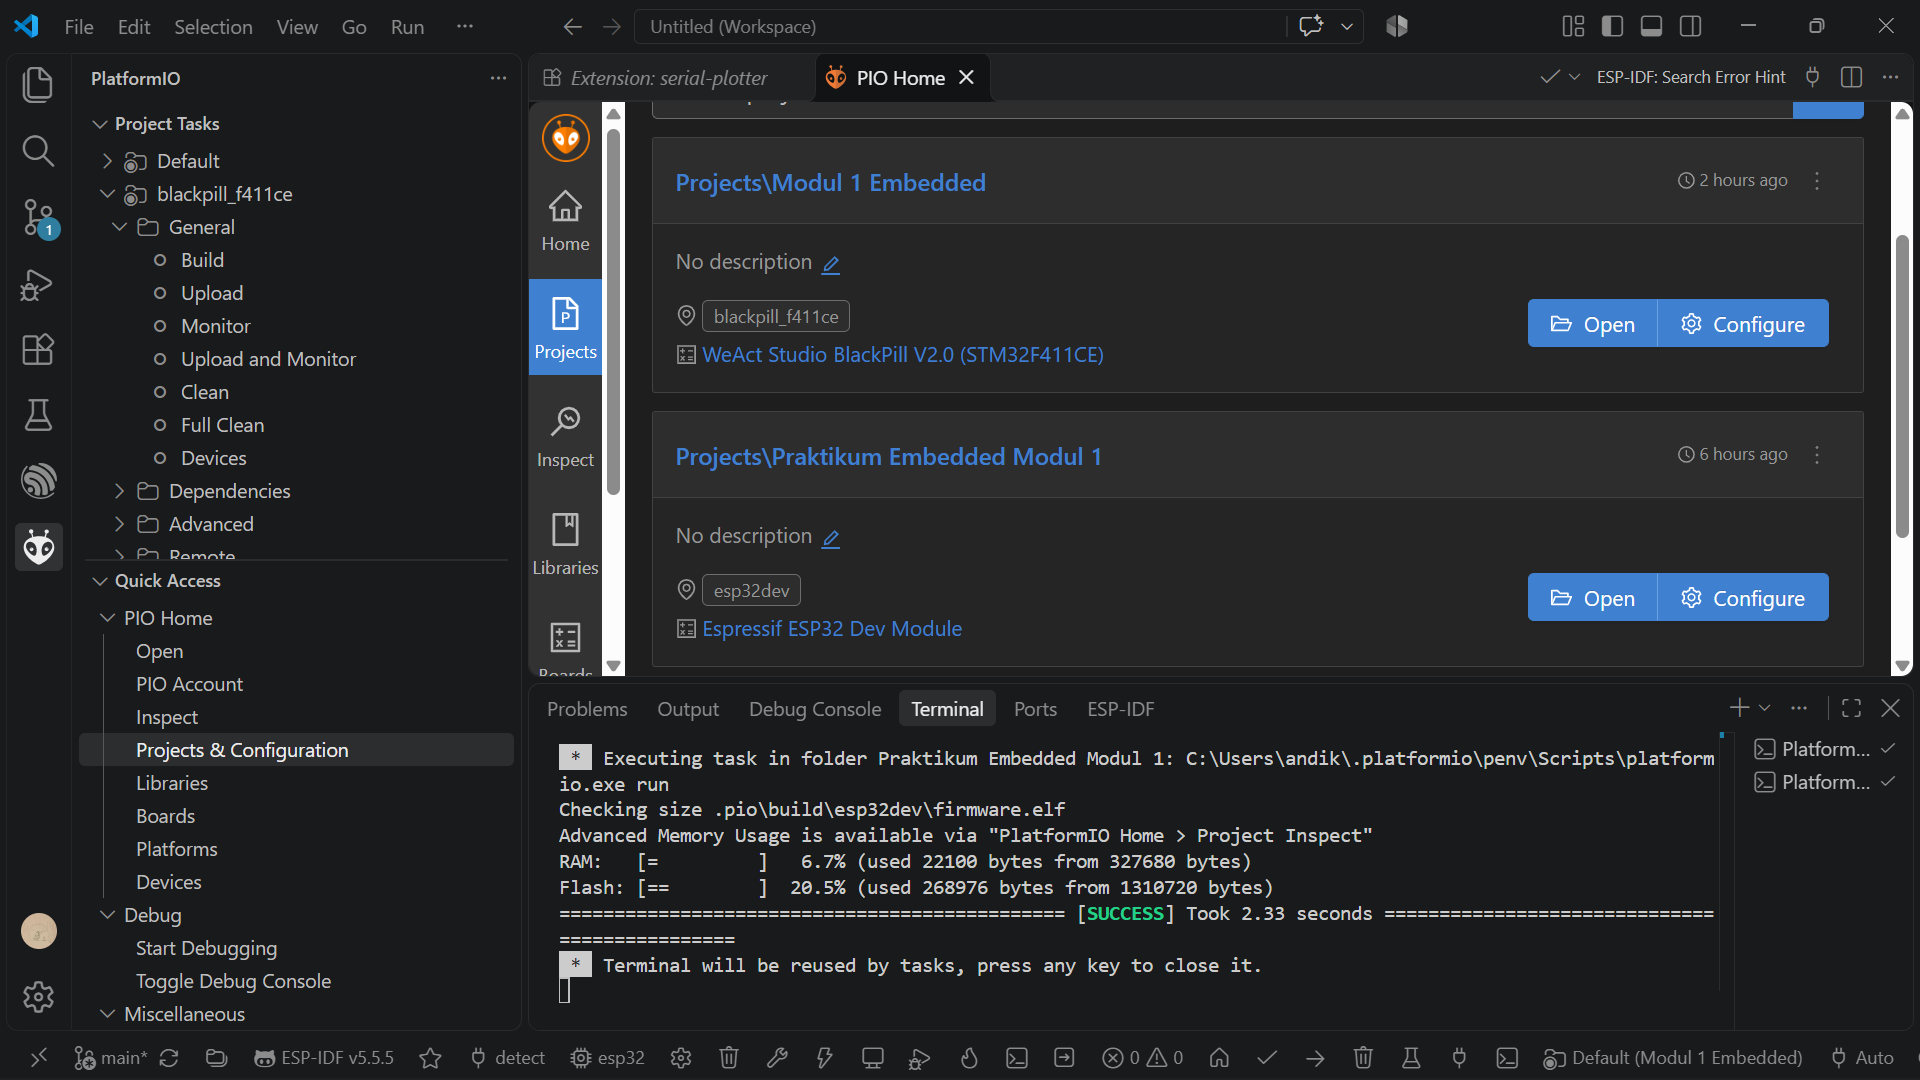
\includegraphics[width=0.5\linewidth]{P1/Screenshot 2026-11-07 081005.png}
        \caption{Platform IO esp success}
        \label{fig:placeholder}
    \end{figure}
    \begin{figure}[H]
        \centering
        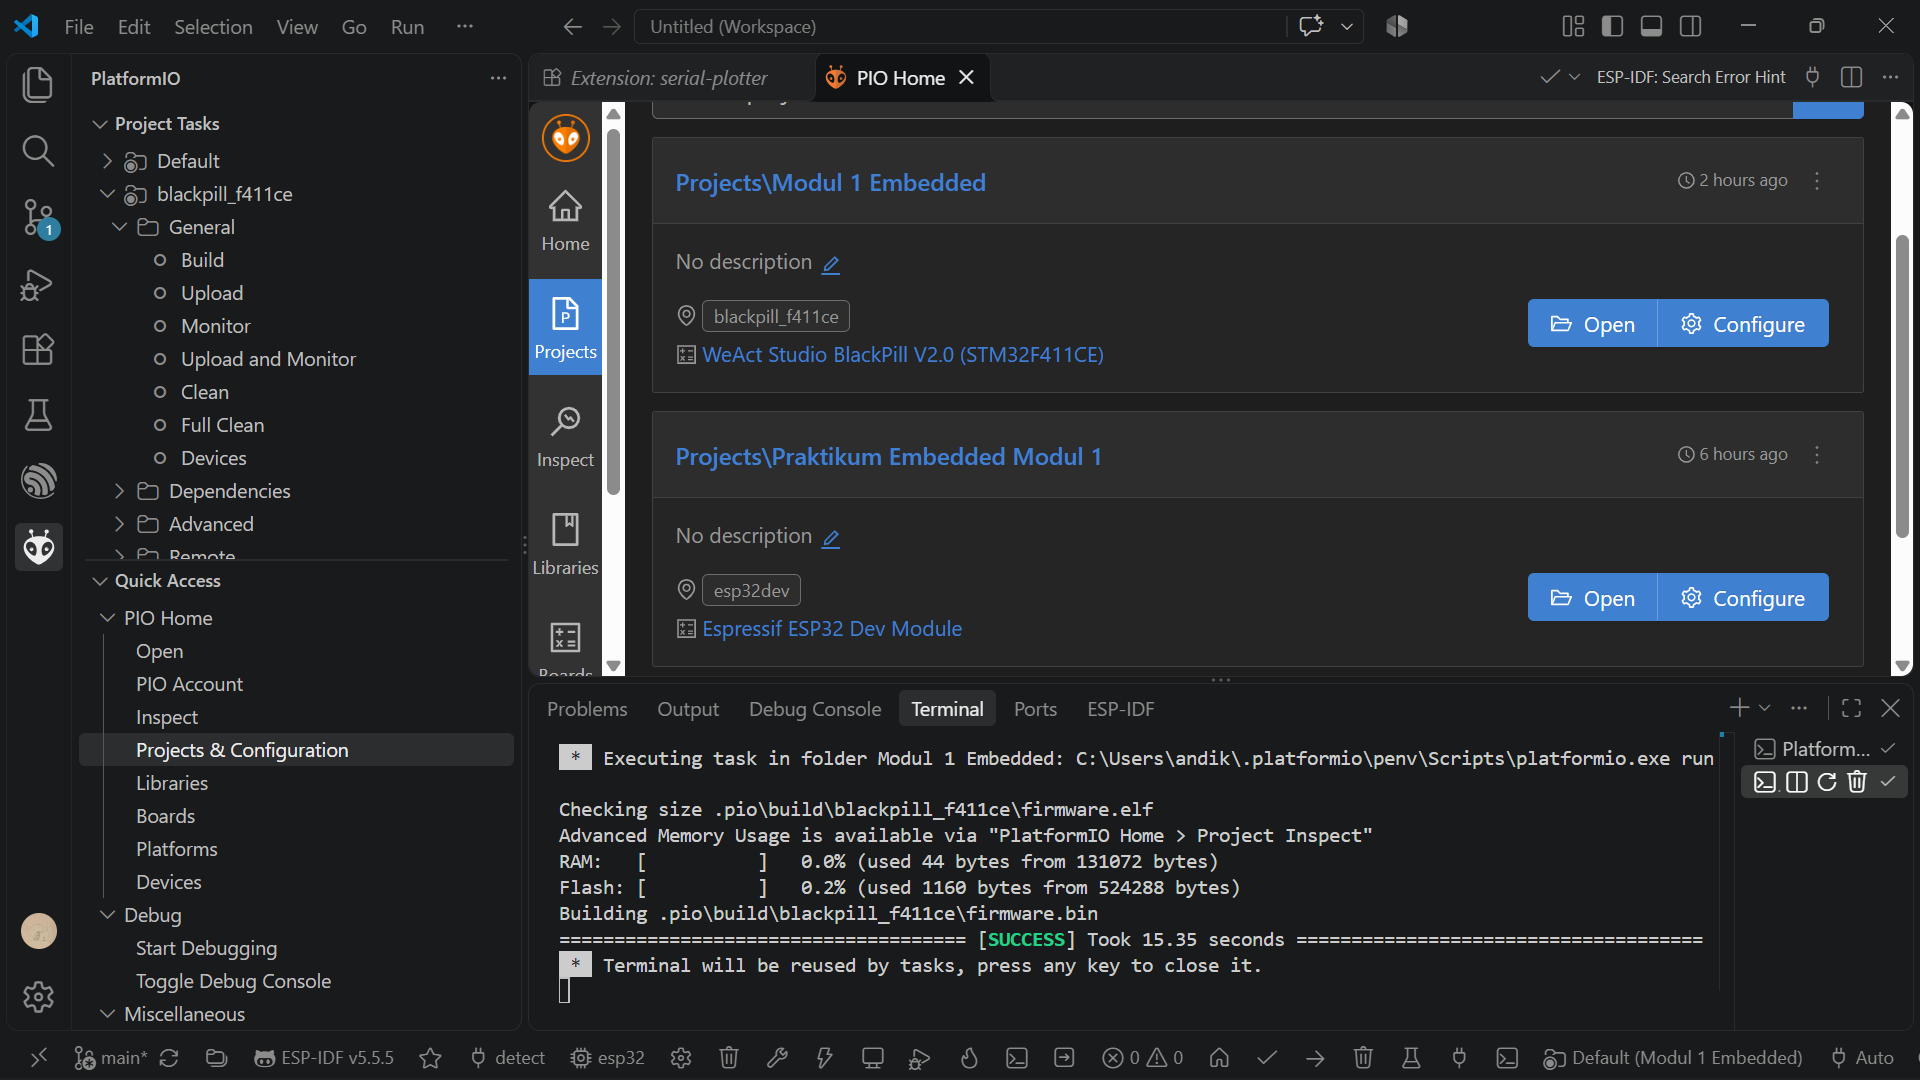
\includegraphics[width=0.5\linewidth]{P1/Screenshot 2026-11-07 081018.png}
        \caption{Platform IO STM Successs}
        \label{fig:placeholder}
    \end{figure}
    \begin{figure}[H]
        \centering
        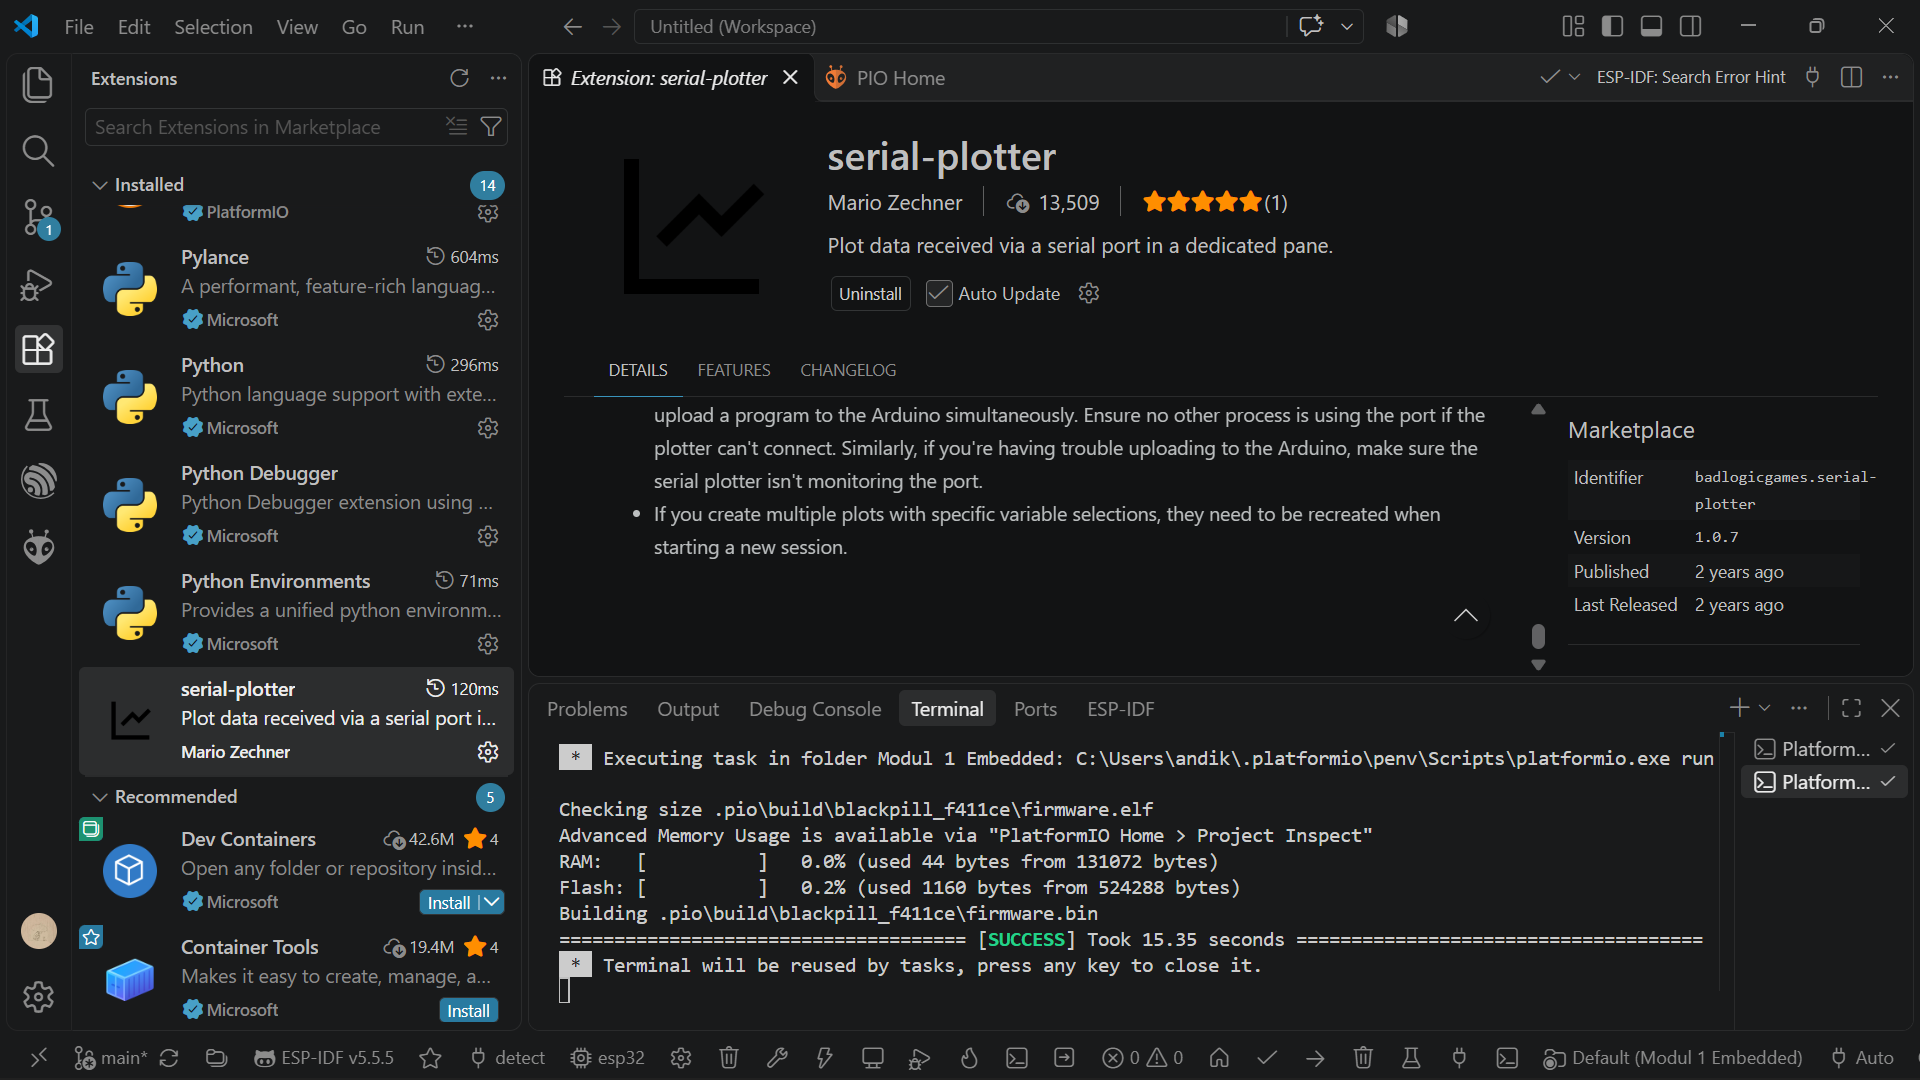
\includegraphics[width=0.5\linewidth]{P1/Screenshot 2026-11-07 081038.png}
        \caption{Plotter Extension}
        \label{fig:placeholder}
    \end{figure}

    
\end{enumerate}